Para podermos derivar a fórmula do Efeito Mínimo Detectável (MDE), precisamos, primeiro, entender o ambiente de nosso experimento. Para isso, começaremos com um simples RCT.\footnote{Um RCT (Randomized Controlled Trial) é um método experimental utilizado em econometria para estimar relações causais. Nesse tipo de experimento, indivíduos ou unidades de análise, como pessoas, escolas ou empresas, são aleatoriamente alocados a um grupo de tratamento, que recebe a intervenção, ou a um grupo de controle, que não recebe. A aleatorização é fundamental para garantir que quaisquer diferenças observadas entre os grupos após o tratamento sejam atribuíveis exclusivamente ao próprio tratamento, eliminando o viés de seleção e assegurando validade interna. Por exemplo, para avaliar o impacto de um programa de bolsas de estudo no desempenho acadêmico, uma população de alunos elegíveis seria dividida aleatoriamente em dois grupos: um que recebe a bolsa e outro que não recebe. Após um período, mede-se o desempenho acadêmico de ambos os grupos, e a diferença média nos resultados reflete o impacto causal do programa. Veja \cite{duflo2007}.} Como motivação, pensaremos num exemplo prático: Avaliar os impactos de estar matriculado em uma escola com ensino técnico. Para isso vamos aleatorizar alunos para entrada na escola com ensino técnico ou em escolar regulares.


%%Athey, S., & Imbens, G. W. (2017). Chapter 3 - The Econometrics of Randomized Experiments. In Handbook of Economic Field Experiments (Vol. 1, pp. 73–140). Elsevier. https://doi.org/10.1016/bs.hefe.2016.10.003

Considere os resultados potenciais, $Y_i(d)$, para os valores de tratamento $d \in \{0,1\}$, os quais serão entendidos nesse exemplo como as notas potenciais do aluno $i$ em uma prova específica.\footnote{Pense numa prova como o Saeb, por exemplo.} O tratamento, $D_i$, será entendido como estar matriculado numa escola de ensino técnico \textbf{específica}, ou seja, se $D_i = 1$, o indivíduo $i$ está matriculado nessa escola específica e, se $D_i = 0$, ele está matriculado em qualquer outra escola. Estamos interessados no Efeito Médio de Tratamento (ATE)\footnote{O ATE (Average Treatment Effect), ou Efeito Médio do Tratamento, é uma medida que quantifica o impacto médio de uma intervenção em uma população, comparando o resultado esperado de quem recebe o tratamento com o de quem não recebe. Em experimentos como RCTs (Randomized Controlled Trials), o ATE pode ser estimado diretamente pela diferença nas médias dos resultados entre os grupos de tratamento e controle, pois a randomização garante que esses grupos sejam comparáveis.}, $\beta = \mathbb{E}[Y_i(1) - Y_i(0)]$, que pode ser interpretado como o efeito causal de estar matriculado nessa escola de ensino técnico específica. Para simplificar o problema, assuma que, se o resultado da loteria for $D_i = 1$, o estudante necessariamente se matricula na escola de ensino técnico e, se $D_i = 0$, ele não consegue se matricular (\textit{perfect compliance}\footnote{Perfect compliance ocorre quando todos os participantes de um estudo seguem exatamente as atribuições de tratamento ou controle conforme planejado, ou seja, quem foi designado para o tratamento o recebe, e quem foi designado ao controle não o recebe. Nesse cenário ideal, os efeitos observados refletem diretamente o impacto causal do tratamento. Na prática, a falta de compliance é comum, e métodos como o ITT ou estimadores instrumentais são usados para lidar com desvios e evitar vieses.}). Ainda, assuma que observamos os resultados de todos os alunos do experimento (não existe atrito),\footnote{Atrito é o termo que se refere a perda de unidades observadas de uma dada amostra. Em nosso exemplo prático, falaríamos que existe atrito caso alguns alunos que estavam em nossa amostra não fizessem a prova da qual estamos interessados em ver o efeito de tratamento. } isto é, observamos os resultados de todos os alunos que participaram do experimento.

Conseguimos identificar o ATE através do $\beta_1$ da seguinte regressão de MQO:\footnote{Mínimos Quadrados Ordinários (MQO) é uma técnica de otimização matemática que procura encontrar o melhor ajuste para um conjunto de dados tentando minimizar a soma dos quadrados das diferenças entre o valor estimado e os dados observados. Veja \cite{angrist2008} para mais detalhes.}
\begin{equation}
    Y_i = \beta_0 + \beta_1 D_i + u_i
\end{equation}

O estimador de MQO para $\beta_1$ é dado pela diferença de médias de $Y_i$ entre o grupo de controle e o grupo de tratamento:
\begin{equation}
    \hat{\beta}_1 = \frac{1}{N_1}\sum_{i:D_i = 1} Y_i - \frac{1}{N_0}\sum_{i:D_i = 0} Y_i
\end{equation}
% Adicionar fórmula do estimador

\noindent em que $N_1$ é o número de alunos tratados e 
$N_0$ é o número de alunos não tratados.\footnote{Em muitos casos, teremos o mesmo número de tratados e controles, isto é, $N_1 = N_0 = N/2$. Desta forma, podemos escrever o estimador de MQO como $\hat{\beta}_1 = \frac{2}{N}\sum_{i:D_i = 1} Y_i - \frac{2}{N}\sum_{i:D_i = 0} Y_i$.} Ao assumirmos homoscedasticidade dos erros, isto é, $\mathrm{Var}(u_i) = \sigma^2$, para todo $i \in \{1,\dots,N\}$, podemos derivar a variância do estimador de MQO:
\begin{equation}\label{varbeta}
    \mathrm{Var}(\hat{\beta}_1) = \frac{1}{p(1-p)}\frac{\sigma^2}{N} 
\end{equation}

\noindent em que $p$ é a proporção de indivíduos no grupo de tratamento e $N$ é o número de indivíduos em nossa amostra. Na próxima subseção, iremos utilizar a fórmula da variância do estimador de MQO para construirmos nosso teste e, a partir dele, iremos derivar o Efeito Mínimo Detectável (Minimum Detectable Effect - MDE).


\subsection{\sc Derivando o MDE}

Gostaríamos de testar se o efeito do nosso tratamento é zero, isto é, $\beta = 0$. Para isso, definimos nossas hipóteses nula e alternativa:
\begin{align*}
        H_0: \beta & = 0\\
        H_1: \beta & \neq 0
    \end{align*}

Com base em nosso exemplo empírico, nossa hipótese nula, $H_0$, significa que o efeito de entrar numa escola de ensino técnico em notas é 0, isto é, o aluno teria a mesma nota tanto numa escola de ensino técnico, quanto numa escola convencional. Já a hipótese alternativa, $H_1$, diz que existe efeito, seja ele positivo ou negativo. Ao desenharmos um experimento, devemos nos preocupar com possíveis erros que podemos cometer ao testarmos essas hipóteses. A tabela \ref{tab:errors} sintetiza os cenários possíveis. 

\begin{table}[h]
    \centering
    \begin{tabular}{l|cc}
         & Não-Rejeita $H_0$ & Rejeita $H_0$ \\\hline
     $H_0$ é verdadeira &  Decisão correta & Erro do tipo I\\
     & ($1-\alpha$)& ($\alpha$)\\
     $H_1$ é verdadeira & Erro do tipo II & Decisão correta \\
     & ($1-\kappa$)& ($\kappa$)\\\hline
    \end{tabular}
    \caption{Erros estatísticos}
    \label{tab:errors}
\end{table}

O Erro de Tipo I, $\alpha$, também chamado de nível de significância, é a probabilidade de rejeitar a hipótese nula quando esta é verdadeira. Já o Erro de Tipo II, $1 - \kappa$, é a probabilidade de não rejeitar a hipótese nula quando a hipótese alternativa é verdadeira. O poder do teste, $\kappa$, é a probabilidade de rejeitarmos a hipótese nula quando a hipótese alternativa é verdadeira, ou seja, estaríamos tomando a decisão correta. Estes conceitos são importantes, pois eles estão diretamente relacionados com o cálculo do MDE. Para testarmos a hipótese de que $\beta = 0$, primeiro definimos o valor de $\alpha$ e $\kappa$. Tipicamente, escolhemos $\alpha = 0.05$. Em seguida, construímos nosso teste estatístico:

    $$
    t = \frac{\hat{\beta}_1 - \beta}{\sqrt{\mathrm{Var(\hat{\beta}_1)}}}
    $$


A estatística $t$ compara o efeito médio calculado com nossa amostra com o efeito verdadeiro. Sob a hipótese de que o efeito não existe, $H_0$, nosso teste se torna:

    \begin{equation}
        t = \frac{\hat{\beta}_1}{\sqrt{\mathrm{Var(\hat{\beta}_1)}}} \stackrel{d}{\longrightarrow} \mathcal{N}(0,1)
    \end{equation}

    Considere um $\Bar{\beta} > 0$, tal que nosso efeito verdadeiro seja $\beta = \Bar{\beta}$, ou seja, nossa hipótese alternativa é verdadeira. Sob a hipótese alternativa, nosso teste terá o formato de uma distribuição normal, porém com sua média deslocada para a direita:

    \begin{equation}
        t = \frac{\hat{\beta}_1}{\sqrt{\mathrm{Var(\hat{\beta}_1)}}} = \underbrace{\frac{\hat{\beta}_1 - \Bar{\beta}}{\sqrt{\mathrm{Var(\hat{\beta}_1)}}}}_{\stackrel{p}{\longrightarrow}\mathcal{N}(0,1)} + \frac{\Bar{\beta}}{\sqrt{\mathrm{Var(\hat{\beta}_1)}}} 
    \end{equation}


\begin{figure}
    \centering
    \includegraphics[width=0.8\linewidth]{Microeconometrics_I.pdf}
    \caption{Distribuições dos testes}
    \label{fig:dist}
\end{figure}

    
Na Figura \ref{fig:dist}, podemos ver as distribuições dos testes sob $H_0$ (preto) e sob $H_1$ (vermelho). O valor $t_{\frac{\alpha}{2}}$ é o valor crítico de nosso teste, isto é, caso o valor absoluto de nosso teste seja maior do que o valor crítico, $| t | > t_{\frac{\alpha}{2}}$, rejeitamos a hipótese nula. Portanto, a área preenchida em azul se refere a região de rejeição do teste. Se nossa estatística $t$ estiver nessa área em azul, significa que a probabilidade do valor verdadeiro de $\beta$ ser 0 é muito baixa. Se nossa hipótese alternativa for verdadeira, estaremos tomando a decisão correta caso $| t | > t_{\frac{\alpha}{2}}$. Portanto, a área preenchida em vermelho se refere ao poder do teste, $\kappa$. Assim, podemos estabelecer a seguinte relação:

\begin{equation}\label{mde1}
    \frac{\Bar{\beta}}{\sqrt{\mathrm{Var(\hat{\beta}_1)}}} - t_{\frac{\alpha}{2}} = t_{1-\kappa}
\end{equation}

Da equação \ref{mde1}, combinando com a fórmula da variância do estimador de MQO obtida na equação \ref{varbeta}, podemos isolar $\Bar{\beta}$ para obtermos o Efeito Mínimo Detectável (MDE):

\begin{equation}\label{mde2}
    MDE := \Bar{\beta} = (t_{\frac{\alpha}{2}} + t_{1-\kappa})\sqrt{\frac{1}{p(1-p)}\frac{\sigma^2}{N}}
\end{equation}

A equação \ref{mde2} nos dá a relação dos parâmetros $\alpha, \kappa, \sigma^2, N$, e $p$ para um valor de $\Bar{\beta}$, que pode ser interpretado como o menor efeito de tratamento que conseguimos detectar dado esses parâmetros. Pesquisadores usualmente assumem  $t_{\frac{\alpha}{2}} + t_{1-\kappa} = 2.8$, uma vez que escolhem $\alpha = 0.05$ e $\kappa = 0.8$.

Note que a fórmula analítica que derivamos para o MDE depende das hipóteses que estamos assumindo. Aqui estávamos assumindo \textit{perfect compliance}, não existência de atrito e homoscedasticidade do erros. Uma hipótese que poderíamos mudar, por exemplo, é a de homoscedasticidade dos erros. Assuma que a variância dos erros dependem do status de tratamento, isto é, $\sigma_d^2 = \mathrm{Var}(Y_i(d))$. Em nosso exemplo prático, isso acontecerá caso acreditemos que a variância das notas na prova para os alunos que foram tratados seja diferente da variância das notas na prova para os alunos que não foram tratados. Isso irá modificar a variância do nosso estimador de MQO, resultando na seguinte expressão para o MDE:

\begin{equation}\label{mde3}
    MDE = (t_{\frac{\alpha}{2}} + t_{1-\kappa})\sqrt{\frac{\sigma^2_1}{N_1} + \frac{\sigma^2_0}{N_0}}
\end{equation}

Na equação \ref{mde3}, $N_1$ e $N_0$ são o número de pessoas tratadas e não tratadas, respectivamente, enquanto que $\sigma_1^2$ e $\sigma_0^2$ são as variâncias de $Y_i$ para os grupos de tratamento e controle, respectivamente. Nas próximas subseções, iremos modificar outras hipóteses e, com isso, iremos derivar o MDE para esses novos contextos.

Quando temos um resultado binário, isto é, $Y \in \{0,1\}$, podemos derivar um limite superior para sua variância

    $$
    \mathrm{Var}(Y) = \mathbb{E}[Y^2] - \mathbb{E}[Y]^2 = p(1-p)
    $$

    em que $p$ é a probabilidade de $Y = 1$. Ao maximizarmos essa expressão, encontramos que $\max \mathrm{Var}(Y) = \frac{1}{4}$. Portanto, podemos derivar um limite superior para o MDE para dados valores de $\alpha, \kappa, N_1, N_0$ como

    $$
    MDE = (t_{\frac{\alpha}{2}} + t_{1-\kappa})\sqrt{\frac{\frac{1}{4}}{N_1} + \frac{\frac{1}{4}}{N_0}}
    $$

Nas próximas seções, iremos mudar diferentes hipóteses a respeito do desenho do experimento, o que fará com que as fórmulas analíticas do MDE mudem.

\subsection{\sc Praticando: Fórmula Analítica}\label{rct_fa}

Existem duas formas de calcularmos o MDE. A primeira é pela fórmula analítica, utilizando das equações que derivamos na seção anterior. Esta é recomendada para quando não temos acessos a dados prévios ao experimento e, portanto, não temos como estimar o desvio padrão de nossa variável de interesse, $Y_i$. Nesse caso, estaremos calculando o MDE em termos de desvios padrões.\footnote{Poderíamos, também, calcular através de simulações sem termos os dados, mas assumindo que conhecemos as distribuições das variáveis. No entanto, não iremos tratar deste método nesse guia.} Caso tenhamos acesso a esses dados, podemos optar por calcular o MDE através de simulações, como veremos mais a frente nesta seção. 

Considere novamente nosso exemplo empírico, em que o tratamento $D_i$, se refere a receber uma vaga numa escola de ensino técnico específica e a variável de interesse, $Y_i$, representa a nota dos alunos numa prova específica. 

Utilizaremos o software R para realizarmos os cálculos. Primeiramente, iremos limpar o ambiente de trabalho e, em seguida, carregaremos o pacote \texttt{tidyverse}. Este pacote irá facilitar a manipulação dos dados e nos auxiliará na criação de gráficos. 

\begin{boxH}
\begin{lstlisting}[language = R]
# Limpar o ambiente 
rm(list=ls())

# Carregando pacotes necessários
library(tidyverse)
\end{lstlisting}
\end{boxH}

O próximo passo consiste em definirmos as variáveis que estarão fixas no cálculo de poder. Da equação \eqref{mde2}, iremos definir $t_{\frac{\alpha}{2}} = 1.96$, pois estaremos trabalhando com um nível de signficância de 5\%; $t_{1-\kappa} = 0.84$, pois desejamos um poder estatístico de 80\%; e $p = 0.5$, isto é, 50\% dos alunos em nossa amostra serão aleatorizados para receberem uma vaga na escola de ensino técnico.

\begin{boxH}
\begin{lstlisting}[language = R]
# Parâmetros para cálculo analítico do MDE

t.kappa = 0.84 # poder de 80%
t.alpha = 1.96 # nível de significância de 5%
P = 0.5 # Porcentagem de tratados de 50%
\end{lstlisting}
\end{boxH}

Agora, com base na equação \eqref{mde2}, iremos criar uma função para calcularmos o MDE para um determinado tamanho da amostra, $N$, utilizando os valores pré-definidos no último bloco de código.  

\begin{boxH}
\begin{lstlisting}[language = R]
# Fórmula do MDE como função de N

MDE = function(N){(t.kappa+t.alpha)*((1/(P*(1-P)))^0.5)*((1/N)^0.5)}
\end{lstlisting}
\end{boxH}

Com essa função criada, podemos calcular o MDE para diferentes tamanhos de amostra. Com $N = 1000$, por exemplo, temos que nosso MDE é de 0.177 desvios padrões.

\begin{boxH}
\begin{lstlisting}[language = R]
# Valor do MDE quando temos N = 1000

MDE(1000)
\end{lstlisting}
\end{boxH}

Uma outra forma de reportarmos os resultados do MDE é através de gráficos. O bloco de código abaixo faz o gráfico da Figura \ref{fig:mdeN}, com os valores do MDE no eixo Y e o tamanho da amostra variando de 500 a 3500 no eixo X. 

\begin{boxH}
\begin{lstlisting}[language = R]
# Gráfico do MDE variando N

ggplot() + xlim(500, 3500) +
  geom_function(fun = MDE, colour = "blue", linewidth = 0.8) +
  labs(y = "MDE", x = "N") +
  theme_classic()
\end{lstlisting}
\end{boxH}

\begin{figure}
    \centering
    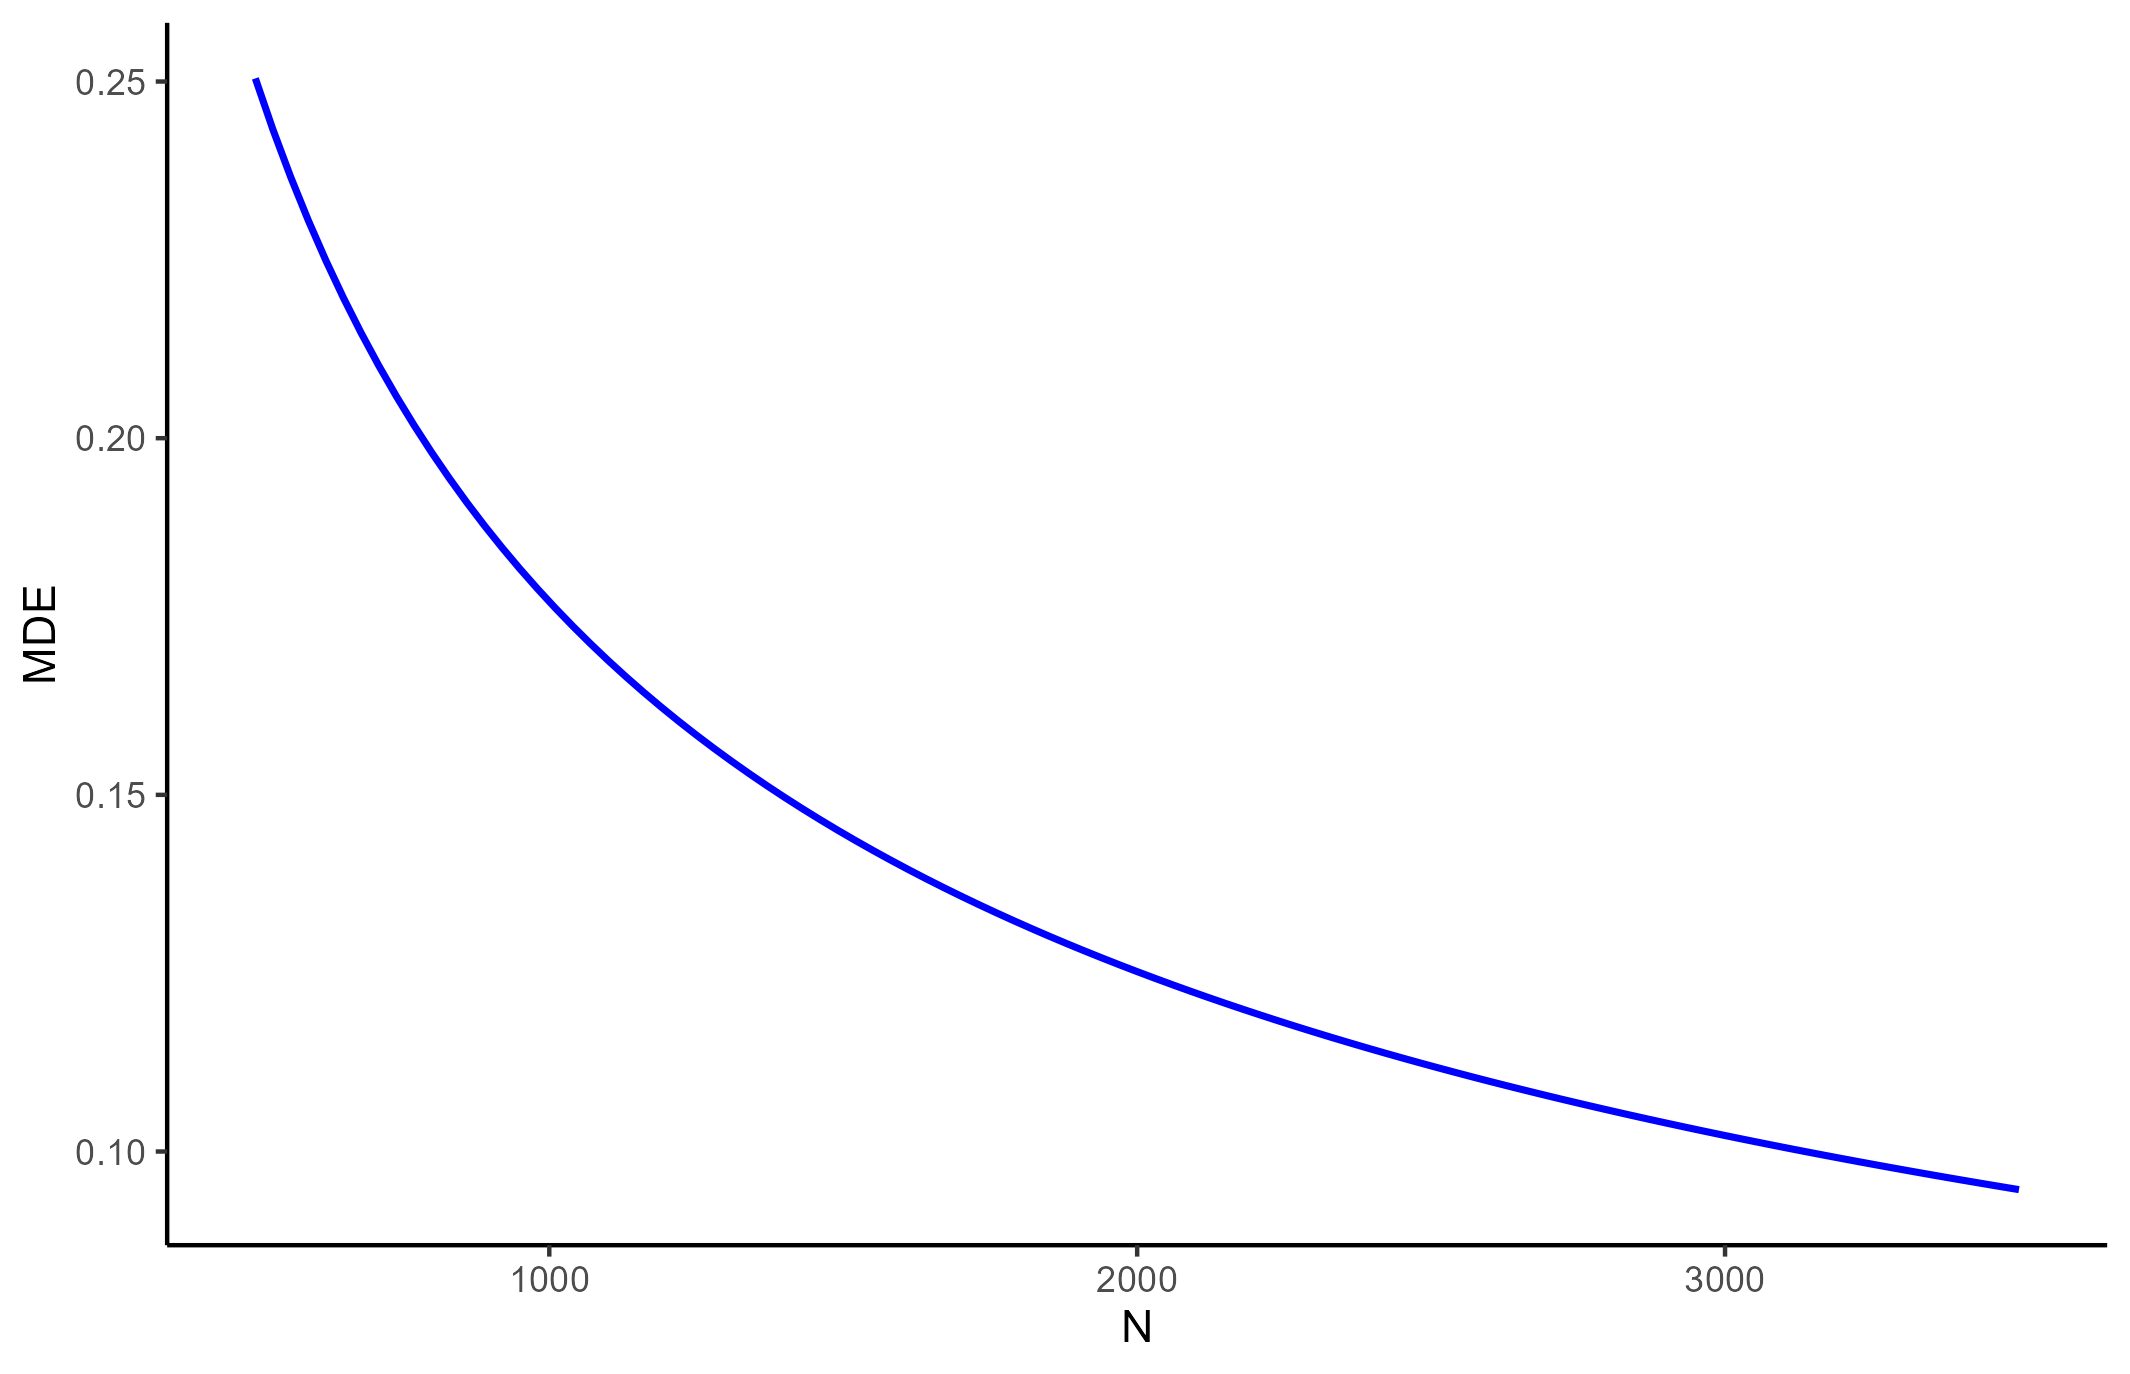
\includegraphics[width=0.8\linewidth]{Figuras/mde.png}
    \caption{Gráfico com valores do MDE variando o tamanho da amostra de 500 a 3500.}
    \label{fig:mdeN}
\end{figure}

Como dito anteriormente, em geral, iremos calcular o MDE em termos de desvio padrão ao utilizarmos a fórmula analítica. Porém, como vimos na seção anterior, quando o $Y_i$ é binário, sabemos o valor máximo que sua variância pode atingir. Assim, no bloco de código abaixo, primeiro definimos o valor máximo da variância, $\sigma^2 = 0.25$, e criamos uma função para o cálculo do MDE máximo no caso binário, utilizando esse parâmetro pré-definido. As últimas quatro linhas do bloco de código fazem o gráfico da Figura \ref{fig:mdebin}. 

\begin{boxH}
\begin{lstlisting}[language = R]
sigma.max = 1/4 # Variância máxima com Y binário

# Fórmula do MDE com Y binário como função de N

MDE.max = function(N){(t.kappa+t.alpha)*((1/(P*(1-P)))^0.5)*((sigma.max/N)^0.5)}

# Gráfico do MDE com Y binário variando N

ggplot() + xlim(500, 3500) +
  geom_function(fun = MDE.max, colour = "blue", linewidth = 0.8) +
  labs(y = "MDE", x = "N") +
  theme_classic()
\end{lstlisting}
\end{boxH}

\begin{figure}
    \centering
    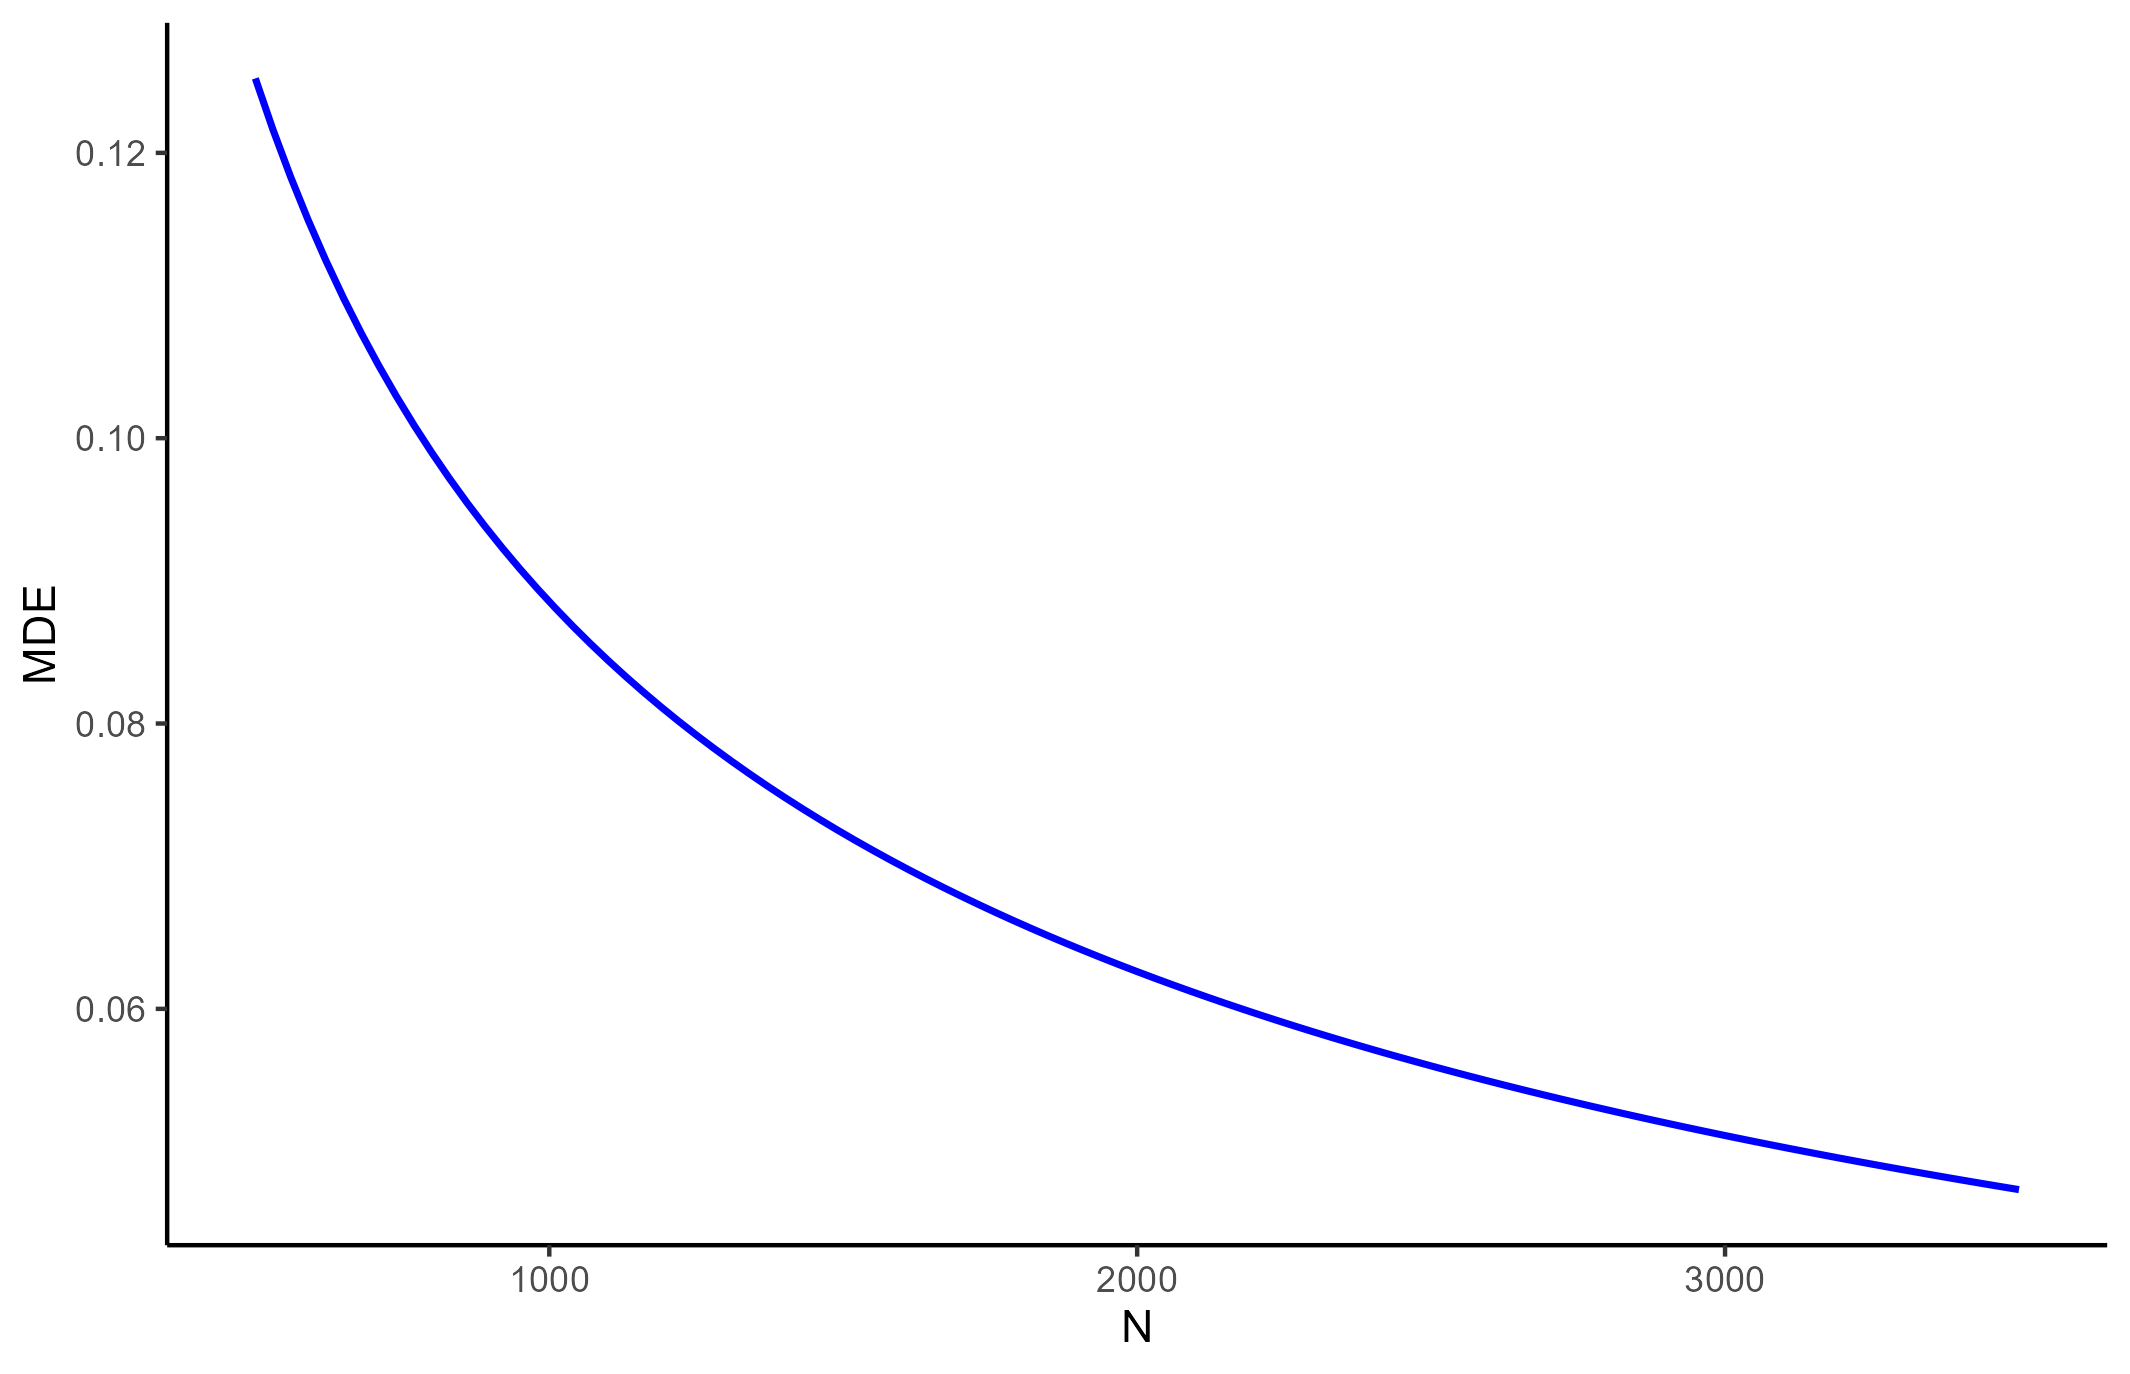
\includegraphics[width=0.8\linewidth]{Figuras/mde_binario.png}
    \caption{Gráfico com valores máximos do MDE no caso em que $Y_i$ é binário, variando o tamanho da amostra de 500 a 3500. }
    \label{fig:mdebin}
\end{figure}

\subsection{\sc Praticando: Simulações}

Através da fórmula analítica do MDE, podemos calculá-lo em termos de desvios padrões, como mostrado na seção anterior. Porém, caso tenhamos acesso a dados de antes da implementação do experimento, conseguimos estimar o desvio padrão através de simulações.

No bloco de código abaixo, iremos limpar o ambiente e carregar os pacotes necessários. Para facilitar a aleatorização dos alunos, iremos utilizar o pacote \texttt{randomizr}.  Para que os resultados sejam reproduzíveis, iremos definir uma \textit{seed},\footnote{As \textit{seeds} de aleatorização são como ``pontos de partida'' para a geração de números aleatórios em um computador. Pense nelas como uma senha ou um código que determina a sequência de números que será gerada. Os computadores, na verdade, não geram números realmente aleatórios, mas sim números pseudoaleatórios, que parecem aleatórios, mas seguem uma lógica definida. Se usarmos a mesma \textit{seed}, o computador produzirá exatamente a mesma sequência de números aleatórios. Isso é útil para garantir que experimentos, simulações ou análises possam ser reproduzidos exatamente da mesma forma em momentos diferentes. Por exemplo, se você rodar um sorteio em um código com uma \textit{seed} específica, e outra pessoa rodar o mesmo código com a mesma \textit{seed}, ela obterá exatamente os mesmos resultados que você.} isto é, um algoritmo de aleatorização, através da função \texttt{set.seed}. Aqui, escolhemos a \textit{seed} 42. Por fim, iremos carregar a base de dados que iremos utilizar, chamada \texttt{base\_rct.csv}, que está dentro da pasta \texttt{Base}.

\begin{boxH}
\begin{lstlisting}[language = R]
# Limpar o ambiente 
rm(list=ls())

# Carregando pacotes necessários

library(tidyverse)
library(randomizr)

# Fazendo com que as simulações se tornem reproduzíveis
set.seed(42)

# Base de dados
base_rct <- read.csv("Base/base_rct.csv")
\end{lstlisting}
\end{boxH}

Agora, iremos simular 100 alocações aleatórias diferentes do tratamento e, a partir disso, calcularemos a média do desvio padrão do estimador do MQO. Cada iteração do \textit{loop} irá \textit{(i)} aleatorizar o tratamento para a nossa amostra, \textit{(ii)} fazer uma regressão de MQO das notas dos alunos, $Y_i$, no tratamento, $D_i$, e, por fim, \textit{(iii)} armazenar o desvio padrão do estimador de MQO num vetor. Para calcularmos o MDE, basta tirarmos a média dos desvios padrões simulados e multiplicarmos pela soma dos valores críticos, $t_{\frac{\alpha}{2}} + t_{1-\kappa} = 2.8$.

\begin{boxH}
\begin{lstlisting}[language = R]
# Criando vetor com 100 entradas para armazenar os erros padrões
se <- c(rep(NA, 100))

# Simulando 100 vezes o erro padrão
for (i in 1:100) {
  
  D <- simple_ra(N = nrow(base_rct), prob = 0.5) # aleatorizando os alunos
  df <- cbind(base_rct, D) # juntando base
  
  reg <- lm(y ~ D, data = df) # regressão
  se[i] <- summary(reg)$coefficients[2,2] # armazenando erro padrão
  
}

# Calculando MDE
MDE = 2.8*mean(se) 
print(MDE)
\end{lstlisting}
\end{boxH}